\documentclass{article}
\usepackage[utf8]{inputenc}
\usepackage{natbib}
\usepackage{graphicx}
\usepackage{subfigure}
\usepackage{amssymb}
\usepackage{amsmath}
\usepackage{amsthm}
\usepackage{mathtools}
\usepackage{mathrsfs}
\usepackage{epstopdf}
\usepackage{booktabs}
\usepackage{setspace}
\usepackage{cases}
\usepackage{dsfont}
\usepackage[colorlinks,linkcolor=blue,anchorcolor=blue,citecolor=blue,urlcolor=blue]{hyperref}

\usepackage{tikz}
\usepackage{forest}

\usepackage[left=1in,right=1in,top=1in,bottom=1in]{geometry}

\newtheorem{example}{Ex}[section]
\newtheorem{defn}{Def}[section]
\newtheorem{thm}{Theorem}[section]
\newtheorem{col}{Corollary}[section]
\newtheorem{rem}{Rmk}[section]
\newtheorem{lem}{Lemma}[section]

\title{ Analysis on the Binary Game }
\author{Yixiang Luo }
\date{\today}

\renewcommand{\baselinestretch}{1.5}
\newcommand{\book}[1]{\textit{#1}}
\newcommand{\C}{\textbf{Comments:}}
\newcommand{\Q}{\textbf{Questions:}}
\newcommand{\pth}[1]{\left( #1 \right)}
\newcommand{\br}[1]{\left[ #1 \right]}
\newcommand{\cur}[1]{\left \{  #1 \right \}}
\newcommand{\vct}[1]{\boldsymbol{#1}}
\newcommand{\mat}[1]{\boldsymbol{#1}}
\newcommand{\abs}[1]{| #1 |}
\newcommand{\norm}[1]{|| #1 ||}
\newcommand{\set}[1]{\left \{  #1 \right \}}
\newcommand{\mon}[1]{\left \langle #1 \right \rangle}
\newcommand{\Rset}{\mathbb{R}}
\newcommand{\pt}[1]{\dot{#1}}


\begin{document}

\maketitle

\begin{spacing}{1.4}


\section{Recurrence relation}
A typical structure of the game looks like the follows.
\begin{center}
  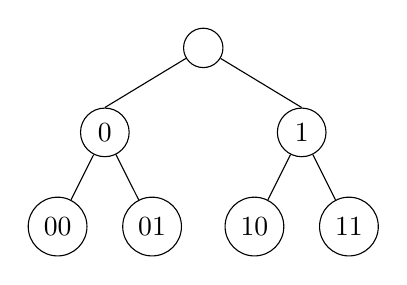
\begin{tikzpicture}[
    node/.style={circle, draw, rounded corners=1mm, text centered, anchor=north, text=black, minimum size=5mm},
    empty/.style={circle, draw=none, text centered, anchor=north, text=black, size=5mm},
    level distance=0.5cm,
    growth parent anchor=south,
    ]
      \node [node] {$~$}
      [sibling distance=2.5cm]
      child{ [sibling distance=1.2cm]
        node [node] (a) {$0$}
        child{
          node [node] {$00$}
        }
        child{
          node [node] {$01$}
        }
      }
      child{ [sibling distance=1.2cm]
        node [node] (a) {$1$}
        child{
          node [node] {$10$}
        }
        child{
          node [node] {$11$}
        }
      };
  \end{tikzpicture}
\end{center}

Each node has a value and it is a random variable. It is easy to show that if the values of all leaf nodes are i.i.d., the values of nodes having the same height are also i.i.d. Assume the leaf nodes have height $0$ and denote the cumulative distribution function (CDF) of the values on nodes having height $i$ as $F_i(x)$, and the corresponding random variable as $V_i$. In the algorithm, the value of a internal node is calculated by taking the maximum or minimum of its two children. So we have
\begin{equation}
  \left\{
  \begin{array}{ll}
    F_{i+1} = F_i^2, & \text{ if take maximum}\\
    F_{i+1} = 1 - (1 - F_i)^2 = 2 F_i - F_i^2, & \text{ if take minimum}
  \end{array}\right.
\end{equation}
Combining the order of playing of the game, we conclude that
\begin{equation}
  \left\{
  \begin{array}{ll}
    F_{i+1} = F_i^2, & \text{ if $i+n$ odd, $i \leq n-1$}\\
    F_{i+1} = 1 - (1 - F_i)^2 = F_i (2 - F_i), & \text{ if $i+n$ even, $i \leq n-1$}
  \end{array}\right.
\end{equation}

\section{Convergence}
Now let's combine two successive updates and derive the relationship as follows.
\begin{numcases}{}
  F_{i+2} = L(F_i) \equiv F_i^2 (2 - F_i)^2, & \text{ if $i+n$ even, $i \leq n-2$} \label{two_step} \\
  F_{1} = F_0^2, & \text{ if $n$ odd} \label{init_ts}
\end{numcases}
What we concern about is the value of the root node, i.e. $F_n$. And the reccurence above is enough for this purpose. If $n$ is even, we apply (\ref{two_step}) on $F_0$ and finally we will reach $F_n$. If $n$ is odd, we apply (\ref{init_ts}) on $F_0$ and then (\ref{two_step}) and finally we will also reach $F_n$.

Now we can state our main result.

\begin{thm} \label{convergence}
The CDF of the value of the root node, i.e. $F_n$, converges pointwisely on even $n$ or odd $n$ sequence. Specifically,
\begin{enumerate}
  \item for even $n$, $F_n$ converge to $\mathds{1}_{x \geq x_1}$, where $F_0(x_1) = 1 - \phi$;
  \item for odd $n$, $F_n$ converge to $\mathds{1}_{x \geq x_2}$, where $F_1(x_2) = F_0^2(x_2) = 1 - \phi$;
\end{enumerate}
where $\mathds{1}$ is the indicator function and $\phi = \frac{\sqrt{5}-1}{2}$ is the Golden ratio.
\end{thm}

\begin{proof}
  \begin{enumerate}
    \item Since $n$ is an even number, after applying $n/2$ times of reccurence (\ref{two_step}) on $F_0$ we get $F_n$. Now let's look at the difference after one reccurence
    \begin{equation}
      D(F_i) = F_{i+2} - F_i = L(F_i) - F_i = F_i^2 (2 - F_i)^2 - F_i
    \end{equation}
    For simplicity, let's ignore the subscript and simply write
    \begin{equation}
      D(F) = F^2 (2 - F)^2 - F.
    \end{equation}
    The function $D(F)$ has only three zeros in $[0, 1]$, which are
    \begin{equation}
      0, \quad 1 - \phi, \quad 1,
    \end{equation}
    and its graph is shown in Figure \ref{D_F}.
    \begin{figure}[!htb] \centering
      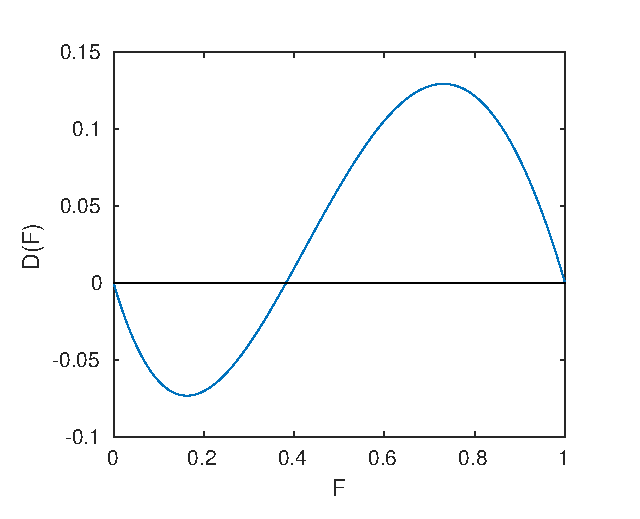
\includegraphics[width=0.4\columnwidth]{figures/D_F.eps}
      \caption{The graph of $D(F)$.}
      \label{D_F}
    \end{figure}

    If $F > 1 - \phi$, after applying the operator $L$ on F, $L(F) > F > 1 - \phi$. So $L^k (F)$ is a strictly increasing function of $k$, if $F > 1 - \phi$, where $L^k (F)$ means applying the operator $L$ $k$ time. In addition, since $L^k (F)$ is a restriction of the CDF $F_{2k}$, we have $L^k (F) \leq 1$. Therefore $F_{2k}(x) \; (F_0(x) > 1 - \phi)$ converges as $k$ goes to infinity.
    Moreover, since there is only one zero of $D(F)$ in $(1 - \phi, 1]$, which is $1$, the only stationary point of $L(F)$ in $(1 - \phi, 1]$ is $1$. Thus $F_{2k}(x) \; (F_0(x) > 1 - \phi)$ converges to $1$.

    Similarly, we have $F_{2k}(x) \; (F_0(x) < 1 - \phi)$ converges to $0$.

    Combining all above, we conclude
    \begin{equation}
      F_n(x) \to \mathds{1}_{F_0(x) \geq 1 - \phi}, \text{ as } n \to \infty, \quad \text{$n$ even}
    \end{equation}

    \item When $n$ is odd, applying the same analysis, but notice now the initial value of the reccurence (\ref{two_step}) is $F_1$, we derive
    \begin{equation}
      F_n(x) \to \mathds{1}_{F_1(x) \geq 1 - \phi} \equiv \mathds{1}_{F_0^2(x) \geq 1 - \phi}, \text{ as } n \to \infty, \quad \text{$n$ odd}
    \end{equation}

  \end{enumerate}
\end{proof}

Then we have the following corollaries immediately.
\begin{col}
  Denote the probability distribution function corresponding to $F_n(x)$ as $f_n(x)$. Then
  \begin{enumerate}
    \item for even $n$, $f_n$ converge to $\delta(x - x_1)$, where $F_0(x_1) = 1 - \phi$;
    \item for odd $n$, $F_n$ converge to $\delta(x - x_2)$, where $F_1(x_2) = F_0^2(x_2) = 1 - \phi$;
  \end{enumerate}
  where $\delta(x)$ is the Dirac delta function.
\end{col}

\begin{col} Denote $\mathbb{E} (V_n)$ and $var(V_n)$ as the expectation and variance of $V_n$ respectively.
  \begin{enumerate}
    \item For even $n$, $\mathbb{E} (V_n) \to x_1$ and $var(V_n) \to 0$, where $F_0(x_1) = 1 - \phi$.
    \item For odd $n$, $\mathbb{E} (V_n) \to x_2$ and $var(V_n) \to 0$, where $F_1(x_2) = F_0^2(x_2) = 1 - \phi$.
  \end{enumerate}
\end{col}

\section{Uniform distribution}
Assume $V_0 \sim U([0, 1])$. Now $F_0(x) = x$ and $F_1(x) = x^2$ ($n$ odd). So
\begin{equation}
  x_1 = 1 - \phi, \quad x_2 = \phi
\end{equation}
and
\begin{enumerate}
  \item For even $n$, $\mathbb{E} (V_n) \to 1 - \phi \approx 0.382$ and $var(V_n) \to 0$.
  \item For odd $n$, $\mathbb{E} (V_n) \to \phi \approx 0.618$ and $var(V_n) \to 0$.
\end{enumerate}

\end{spacing}
\end{document}
